\chapter {Descripción de Ambienta2MX}
  \section {¿Qué y para qué es Ambienta2MX?}
    \paragraph {\underline{Ambienta2MX} es el nombre de la plataforma que pretende formar parte de una macro solución orientada a la estandarización de datos geoespaciales que el INEGI y otras instituciones públicas tienen en su haber.}
    \paragraph{Actualmente no existe un estándar de datos geográficos a nivel nacional. Han existido aproximaciones mediante concursos que instituciones públicas como el INEGI ha publicado, o simplemente han existido propuestas que han brindado una solución incompleta a la unión y manejo de información geográfica, geodésica, hidrográfica, climática, topográfica, etc.}
    \paragraph{\underline{Ambienta2MX} toma parte de todo el problema y propone una infraestructura lógica para afrontar la estandarización de variables ambientales y algunos índices de contaminación. Esta información actualmente se encuentra en formatos muy rudimentarios como textos planos sin algún protocolo o definición para su interpretación.}
    \paragraph{Sistemas semejantes, por ejemplo, el \textbf{Servicio Meteorológico Nacional} carece de algún recurso del cual se puedan realizar consultas que no sea mediante su portal web, esto trae problemas directos de compatibilidad con otros sitemas.}
    \paragraph{Un caso semejante se tiene con la información que la \textbf{Conagua} maneja en sus centrales meteorológicas a lo largo del país, los datos que brindan se actualizan de forma periodica y el único medio de acceso es a través de una página de internet que devuelve archivos en formato de texto u hojas de cálculo.}
    \paragraph{Los impedimentos antes mencionados conllevan a situaciones tan triviales como la consulta de datos para algúna región o punto específico del territorio nacional, al existir diversas fuentes no es posible tener un compendio del cual tomar la información que más sea conveniente.}
    \paragraph{Si a este problema se le añade que los datos carecen de un estandar, se puede visualizar el punto en que intentar manipular o tratar los datos se vuelve una tarea complicada y en exceso tediosa.}
    \paragraph{Considerando dichos problemas \underline{Ambienta2MX}, propone un estandar de datos climáticos tomando como referencia diversas fuentes y adaptando los tipos de datos a tecnologías y tendencias actuales, brindando así una mayor portabilidad y simplicidad en la consulta de información.}
  \newpage
  \section{Diagrama de Ambienta2MX}
    \paragraph{\underline{Ambienta2MX} constará de varios módulos que trabajarán de forma conjunta para satisfacer la necesidad de tener un estandar y un repositorio de datos climáticos a nivel nacional.}
    \paragraph{Al brindar un sistema modularizado, se genera de forma directa un impacto en el proceso de análisis, desarolló e intengración. Éste tipo de modelo describe de una forma sencilla los componentes necesarios para solventar la demanda a la que se encontrará sometida la plataforma.}
    \paragraph{A continuación se muestra el diagrama a bloques de \underline{Ambienta2MX} (véase Figura 7.1), todos los módulos, recursos y bases de datos serán descritos de forma posterior.}
  \newpage
    \begin{landscape}
      \begin{figure}[h!]
      \centering
      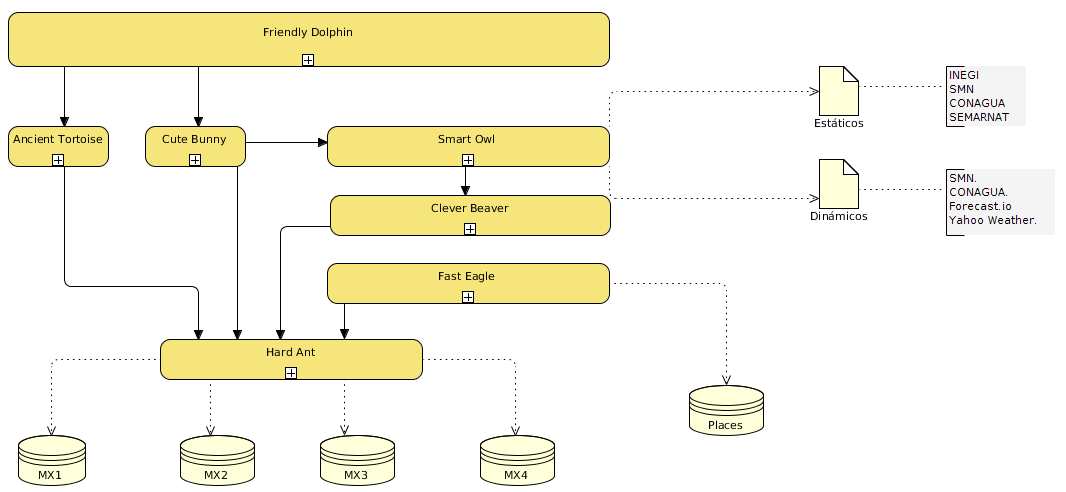
\includegraphics[width=22.5cm,height=12cm]{./images/DiagramaAmbienta2MX.png}
      \caption{Módulos y estructura de Ambienta2MX}
    \end{figure}
    \end{landscape}
  \newpage
    \paragraph{Cómo se apreciar en el diagrama, además de los gestores de bases de datos, \underline{Ambienta2MX} se encuentra dividido en siete módulos básicos:}
    \begin{itemize}
    \item Friendy Dolphin.
    \item Cute Bunny.
    \item Smart Owl.
    \item Fast Eagle.
    \item Hard Ant.
  \end{itemize}
    \paragraph{En el mismo diagrama se pueden observar las fuentes que proporcionarán la información ya sea a un nivel estático, por ejemplo, carta climática anual de algún municipio del territorio nacional; o bien, recursos que se actualizan de forma periodica como son los datos que provee el Servicio Meteorológico Nacional.}
    \paragraph{Se condieran cinco bases de datos, \emph{MX1, MX2, MX3, MX4, Places}. Todas las bases del tipo MX contarán con la información de variables ambientales así también de los índices de contaminación de las zonas que conforman al territorio nacional.}
    \paragraph{Para el caso de \emph{Places}, la base será usada como un macro índice cartográfico del territorio nacional, es decir, esta base será la referencia a nivel latitud, longitud y altitud para ubicar los datos que requieran ser procesados.}
    \paragraph{Todas las bases se encontrarán funcionando bajo un modelo de base de datos documental teniendo una alimentación bajo demanda, es decir, el contenido gestionado irá aumentando conforme las éstos vayan siendo solicitados.}
\chapter{Módulos de Ambienta2MX}
    \section{Friendly Dolphin}
  \subsection{Definición y objetivos}
    \paragraph{Éste módulo es el encargado de brindar la información procesada al usuario a través de una página de internet (véase Figura 8.1). Es el módo visual que los usuarios finales tendrán para poder interactuar con el ecosistema Ambienta2MX.}
    \paragraph{Se presenta cómo un módulo web que consumirá la información procesada y almacenada por las cuatro bases (MX1,MX2,MX3,MX4) y la base de soporte (Places).}
    \begin{figure}[h!]
        \centering
          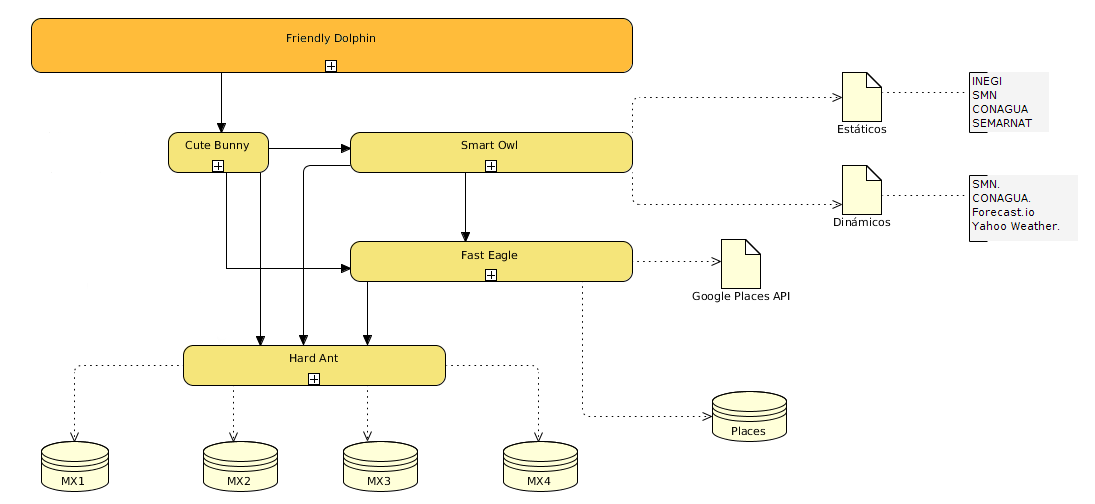
\includegraphics[width=\textwidth]{./images/DiagramaAmbienta2MX_FriendlyDolphin.png}
        \caption{Friendly Dolphin, Módulo de Ambienta2MX.}
    \end{figure}
    \paragraph{La principal función es la de consulta y visualización de datos. Es la capa más expuesta y visual de Ambienta2MX ya que es la que tendrá interacción directa con usuarios no técnicos, sin embargo, contará con los procesos necesarios para poder extraer información de las demás plataformas en formatos convencionales cómo JSON o CSV para uso posterior del usuario.}
  \subsection{Alcances}
    \paragraph{Interactúa de forma directa con el bloque \textbf{\emph{Cute Bunny}}, que forma parte de la segunda capa de exposición de datos de Ambienta2MX. Se comunica con los demás módulos mediante servicios de tipo REST que funcionan bajo el patrón de convención sobre configuración\cite{8}, brindando así una gran compatibilidad con éstos además de disminuir el tiempo de desarrollo debido a que no es necesario generar código único y se opta por la reutilización de éste además de apoyarse con el uso de bibliotecas que siguen el mismo método de trabajo.}
    \paragraph{Friendly Dolphin sólo puede ser visto como una herramienta de consulta, no podrá ser visto cómo un utensilio de análisis de datos climatológicos, es por ello que muestra la información en mapas, gráficas y detalles de la consulta.}
  \subsection{Restricciones}
    \paragraph{Éste módulo se ve limitado por la API de Google Maps para la visualización de la información, ya que las consultas resultan limitadas en su versión gratuita, sin embargo, la cantidad es suficiente para demostrar la aplicación de los datos en una herramienta de visualización. Las restricciones estan definidas a 25,000 solicitudes por día y limitada a un segundo por petición o usuario.}
    \paragraph{La vista también cuenta con cierta limitantes, sólo podrá ser visualizada en navegadores con Internet Explorer 11+, Mozilla Firefox 20+ y Google Chrome 20+}
  \subsection{Arquitectura}
    \paragraph{Friendly Dolpin contará con varios procesos y módulos a ser desarrollados (véase Figura 8.2). Éste módulo se desarrollará usando tecnologías cómo HTML, Javascript y CSS, además de contar con un ciclo continuo de desarrollo usando herramientas de apoyo cómo Yeoman, Gulp para el maquetado y gestión de tareas comunes en projectos de tipo web.}
    \paragraph{Se hará uso del servidor interno que ofrece Gulp junto con las tareas y gestión de bibliotecas de terceros. En cuanto al desarrollo de los estilos necesarios para las vistas se implementará Bootstrap cómo maquetado CSS y finalmente el manejo de vistas, peticiciones y lógica dentro del navegador de los clientes se implementará un patrón de tipo SPA (Single Page Application)\cite{36} desarrollado por el equipo de trabajo.}
    \begin{figure}[b!]
      \centering
        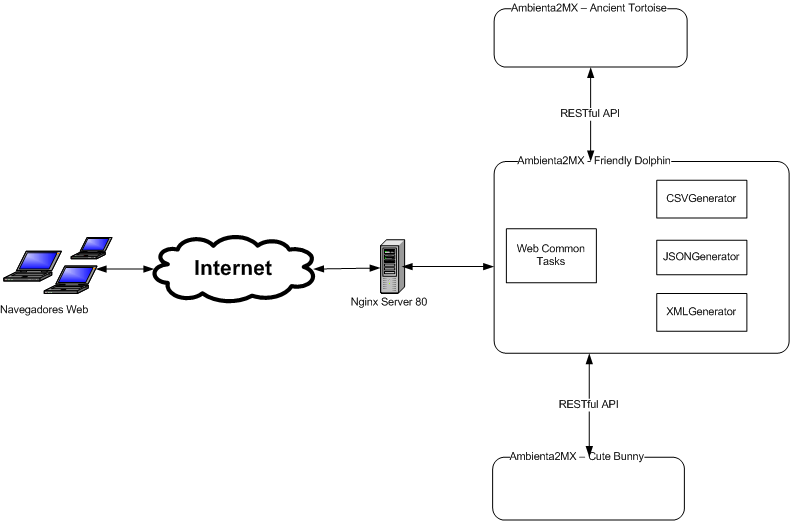
\includegraphics[width=\textwidth]{./images/DiagramaFriendlyDolphin.png}
      \caption{Diagrama General de Friendly Dolphin}
    \end{figure}
  \subsection{Factibilidad}   
    \paragraph{Se decidió cambiar de framework en las vistas, se quitó la implementación de EmberJs del proyecto y se optó por simplemente la ideología que éste tiene, considerando un patrón SPA\cite{36} mínimo ya que el framework antes mencionado contaba con demasiadas características que no iban a ser implementadas sin embargo el framework hace uso de estas.}
    \paragraph{Se optó por seguir esa ideología brindando la flexibilidad necesaria que consideró el equipo de trabajo para cumplir con el objetivo de tener una página dinámica que convive con los demás módulos de Ambienta2MX.}
    \paragraph{A continuación se muestran las características principales de cada tecnología:}
    \paragraph{``EmberJs''}    
    \begin{itemize}
      \item Manajo de un patrón SPA.
      \item Trabajo y desarrollo utilizando Convenció sobre configuración.
      \item Control de rutas, controladores, modelos, vistas, pruebas y dependencias externas.
      \item Implementación de plantillas (templates).
      \item Uso de AJAX como forma de interacción con servicios externos.
    \end{itemize}
    \paragraph{``Servicio Generado por el Equipo de Ambienta2MX''}    
    \begin{itemize}
      \item Uso de AJAX como forma de interacción con servicios externos.
      \item Manejo básico de templates para vistas.
      \item Control de rutas y datos adquiridos del servidor.
    \end{itemize}
    \paragraph{Cómo puede verse, el framework EmberJs contiene más caracteristicas que las necesarias para el desarrollo del proyecto, es por eso que decidió adaptarse esa misma ideología haciendo uso de  un framework mínimo creado por el equipo de Ambienta2MX totalmente adecuado a las necesidades que tiene en éste caso el módulo Friendly Dolphin.}
  \subsection{Pruebas y Capturas de pantalla}
    \paragraph{Para este módulo se realizaron pruebas funcionales indicando el flujo básico de información que un usuario común seguiría. Las pantallas básicas se muestran a continuación y la información de las pruebas pueden ser visualizadas en el anexo en este documento.}
    \begin{figure}[b!]
      \centering
        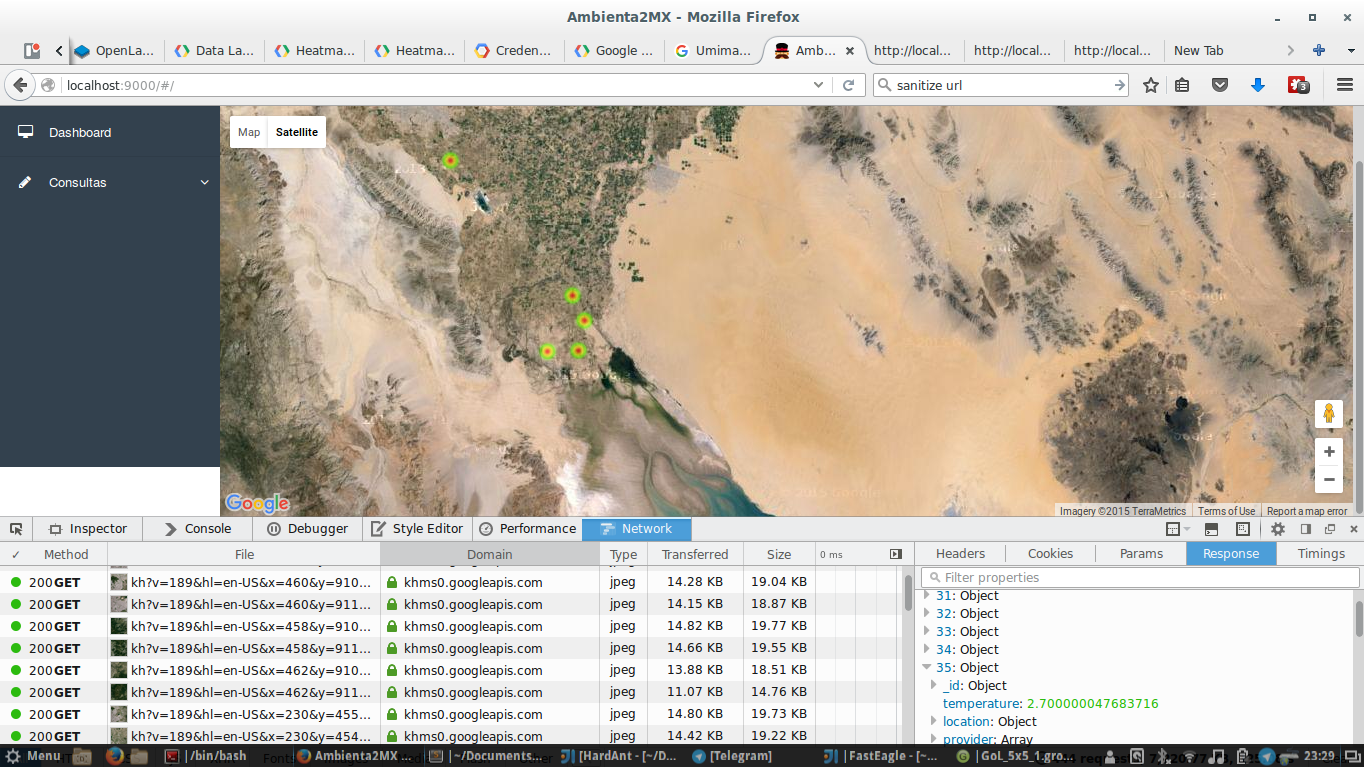
\includegraphics[width=\textwidth]{./images/CapturaFriendlyDolphin}
      \caption{Mapas de Calor, Friendly Dolphin}
    \end{figure}
    \paragraph{Cómo se puede visualizar en la imagen anterior los datos de clima de ciertas regiones del país, en este caso en el área de Baja California, utilizando un concepto llamado HeatMap (Mapa de Calor) que nos permite la transposición de un mapa de Google y los datos climatólogicos recolectados por el sistema de Ambienta2MX. Ésta vista puede ser vista por medio del formulario de busqueda ubicado en la parte superior de las vistas que fueron generadas (véase Figura 8.4).}
    \begin{figure}[b!]
      \centering
        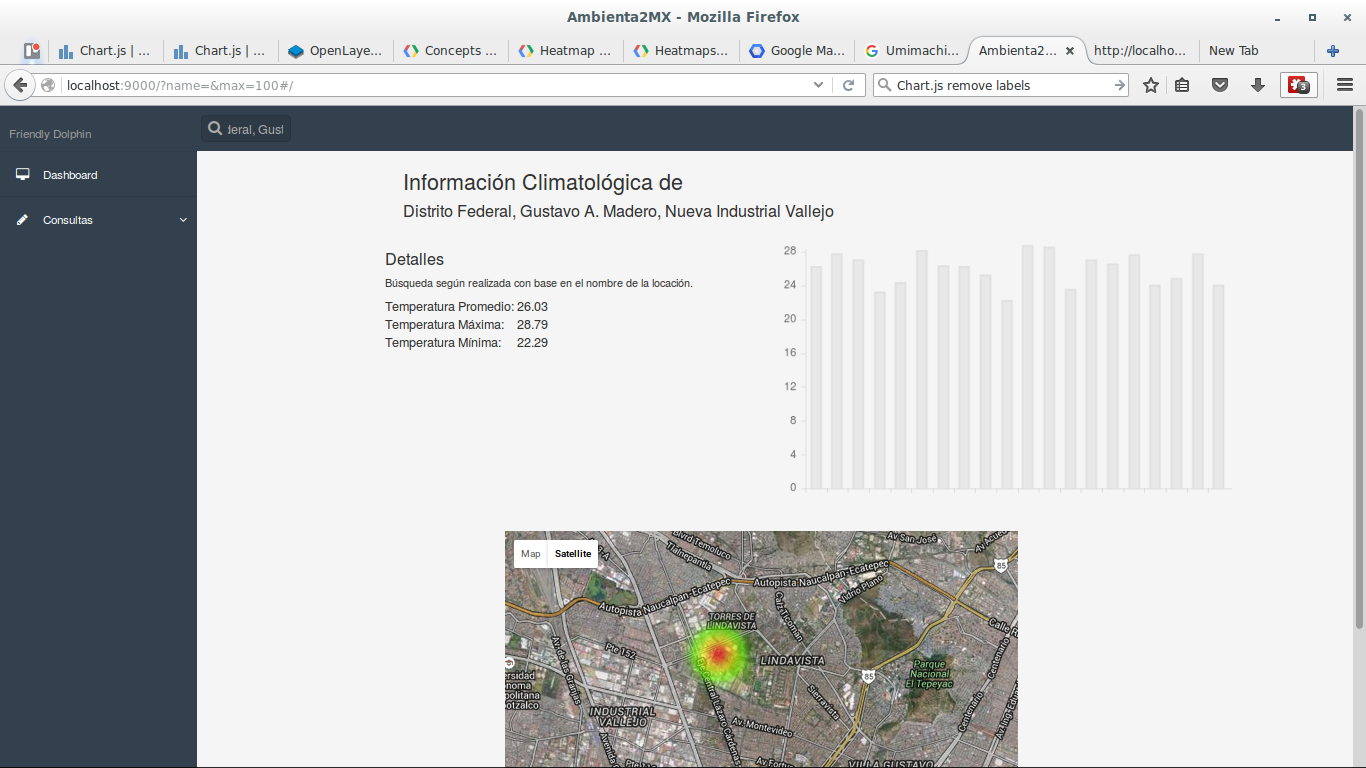
\includegraphics[width=\textwidth]{./images/CapturaFriendlyDolphin2}
      \caption{Tablas e información de clima, Friendly Dolphin}
    \end{figure}
    \paragraph{También puede ser visualizada la información en forma de gráfica de barras, considerando en este caso el área de estudio que es el Distrito Federal, principalmente la parte norte de la capital.}
    \paragraph{El mapa de calor (HeatMap) se traslapa con la vista satelital que nos brinda el servicio de Google Maps. En esta captura se puede apreciar de mejor manera el espectro de temperatura en el área en cuestión, mostrando de un color rojo las áreas con el más alto índice de temperatura y disminuyendo a un color verde en las zonas donde la sensación termica fue menor.}
    \begin{figure}[b!]
      \centering
        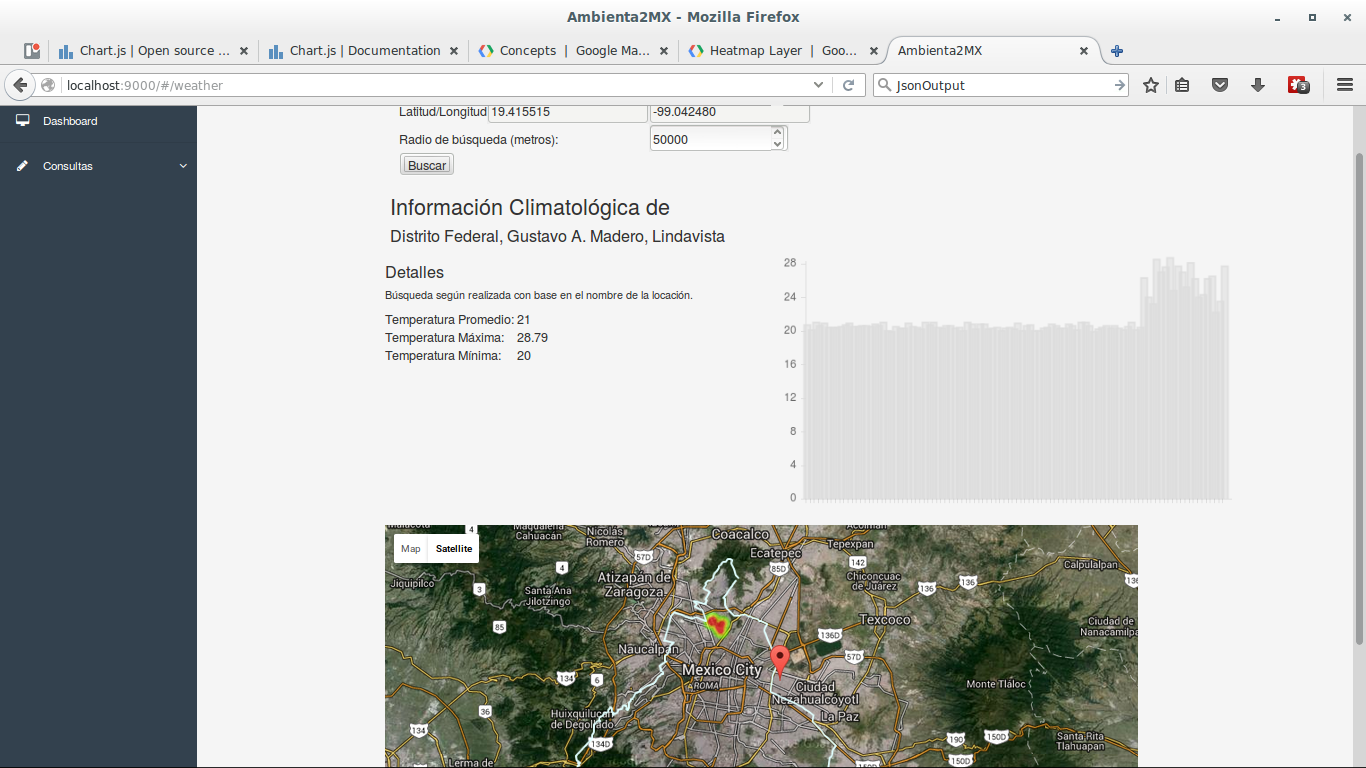
\includegraphics[width=\textwidth]{./images/CapturaFriendlyDolphin3}
      \caption{Tablas e información de clima, Friendly Dolphin}
    \end{figure}
    \paragraph{Cómo puede verse en la siguiente imagen, también se cuenta con una consulta que toma como base un ``Marker'' cólocado por el usuario e índicando el radio de búsqueda en metros. Con ello, el servicio recorrerá las bases de tipo MX para poder encontrar los datos climatológicos o bien de contaminación que cumplen con el criterio de proximidad tomando la información Latitud/Longitud existente en el mapa.}
    \paragraph{Éste tipo de búsqueda resulta util cuando se desea analizar los datos de un área delimitada por un círculo. El ejemplo muestra los datos a 50 kilométros de Ciudad Nezahualcóyotl (Estado de México), coincidiendo con datos de prueba (ubicados en la delegación Gustavo A. Madero), demostrando la funcionalidad de la búsqueda.}
    \paragraph{La información que hace referencia a variables de contaminación ambiental cuenta con pantallas análogas a las mostradas.}
    \paragraph{Las pruebas funcionales fueron ejecutadas utilizando el framework \textbf{iMacros}, a continuación se muestra la rutina que indica la consulta de un lugar y se muestra en la pantalla.}
    \begin{figure}[b!]
      \centering
        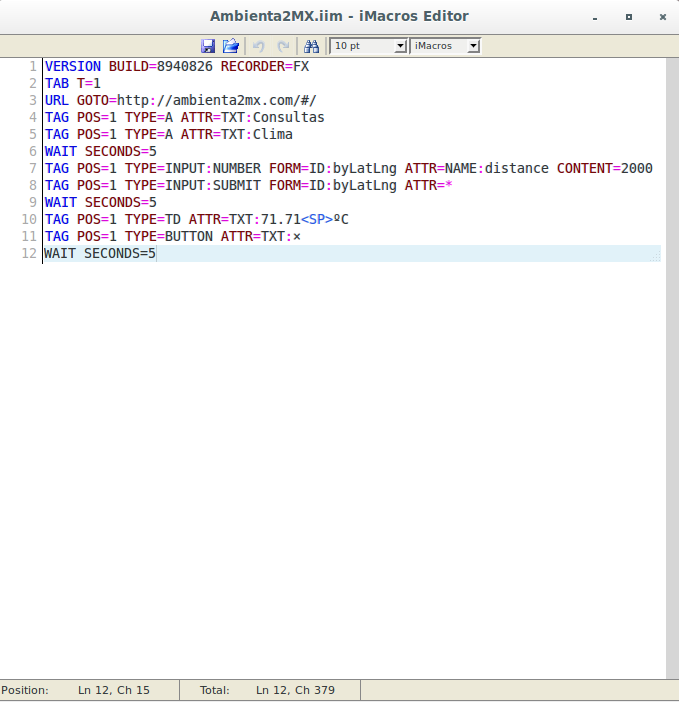
\includegraphics[width=\textwidth]{./images/funcional}
      \caption{Código de prueba funcional}
    \end{figure}
    \section{Cute Bunny}
  \subsection{Definición y objetivos}
    \paragraph{El módulo \textbf{\emph{Cute Bunny}} es parte medular para la comunicación con otros sistemas. Cute Bunny es el encargado de proporcionar los respectivos servicios de tipo REST a otros sistemas o módulos que deseen consultar la información almacenada en las respectivas bases de tipo MX (véase Figura 8.5).}
    \paragraph{Cute Bunny tiene como objetivo unir y establecer la comunicación inicial entre los módulos de Ambienta2MX y la vista del usuario final, proporcionada por el módulo Friendly Dolphin. A continuación se muestra su ubicación con el diagrama general de Ambienta2MX.}
    \begin{figure}[h!]
        \centering
          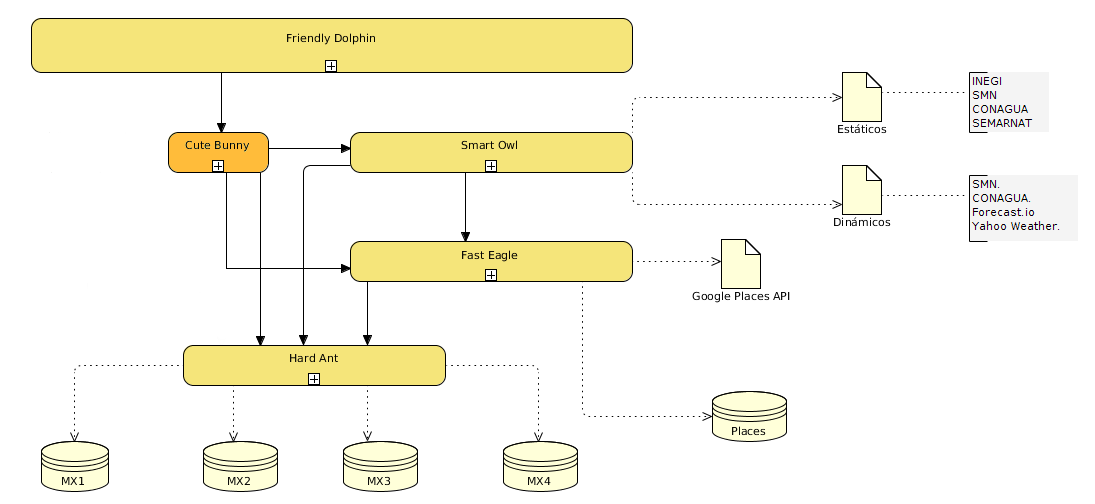
\includegraphics[width=\textwidth]{./images/DiagramaAmbienta2MX_CuteBunny.png}
        \caption{Cute Bunny, Módulo de Ambienta2MX.}
    \end{figure}
    \paragraph{Cute Bunny interactúa con todos módulos de Ambienta2MX, Smart Owl, Hard Ant y Fast Eagle. La interacción con estos surge debido a que Hard Ant es el encargado de gestionar el acceso a las bases de datos de tipo MX y Smart Owl brindará y dará solución a las busquedas que no se encuentren en las bases de tipo MX, es decir, tratará de encontrar la información que Cute Bunny le solicitó para guardarla en algunas de las bases y posteriormente regresar el resultado al solicitante, en el caso de Fast Eagle, para la búsqueda de locaciones en la base de datos Places.}
  \subsection{Alcances}
    \paragraph{Considerando el objetivo primordial, qué es el de comunicar y unir, su único alcance es el de mantener la conexión de forma transparente entre los módulos y permitir la interacción como si todos se encontraran dentro de una misma máquina o servicio único; esto con la finalidad de brindar el acceso a los datos mediante una API de tipo REST libre del contexto y alcance de cada módulo.}
    \paragraph{Considerando la aplicación de un servidor como Nginx, se puede permitir expandir la funcionalidad sin mostrar al usuario la existencia de diversos sistemas trabajando bajo la misma dirección, es una de sus más grandes bondades.}
  \subsection{Restricciones}
    \paragraph{Una de las principales limitantes de éste módulo se ve reflejada en el negocio, debido a que carece de una capa lógica o de procesos entonces se terminó por delegar la información y la lógica a los otros proyectos involucrados.}
    \paragraph{Para éste módulo se decidió hacer uso de un servicio tipo proxy que sólo se encarga de mantener la transparencia como una API única, carece totalmente de un sentido en el negocio y puede ser cambiado por algún otro tipo de servidor web.}
  \subsection{Arquitectura}
    \paragraph{A continuación se mostrará el diagrama por bloques que define la estructura de Cute Bunny.}
      \begin{figure}[b!]
        \centering
        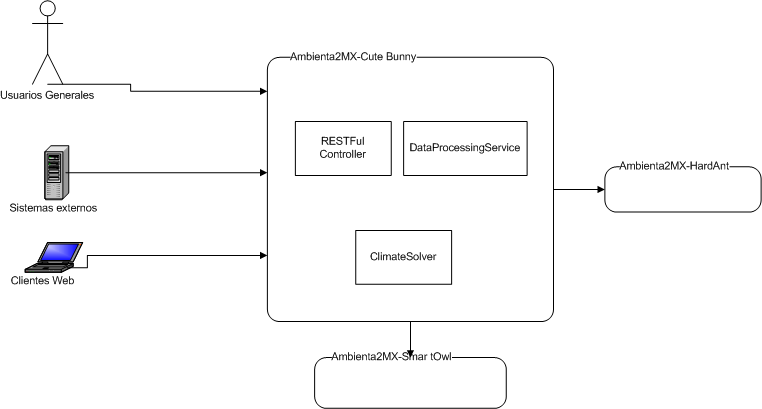
\includegraphics[width=\textwidth]{./images/DiagramaCuteBunny.png}
        \caption{Diagrama General de Cute Bunny}
      \end{figure}
    \paragraph{Como puede ser visualizado, funge como el pegamento de todos los módulos para que éstos puedan ser accedidos desde la vista (Friendly Dolphin), o bien, que servicios de externos puedan alimentarse de la información climatológica obtenida por el sistema Ambienta2MX (véase Figura 8.6).}    
  \subsection{Factibilidad}      
    \paragraph{Originalmente se tenía pensado realizar la implementación y unión de todos los módulos del negocio de Ambienta2MX utilizando la tecnología Grails, sin embargo, se dió un cambio drástico debido a que el framework realmente no sería utilizado al 100\%, lo cual nos permitió visualizar el problema desde un punto más de DevOps \cite{38}, optando por la aplicación del servidor nginx como pieza para la unión del sistema.}
    \paragraph{A continuación se muestran las características principales de cada tecnología:}
    \paragraph{``Grails''}    
    \begin{itemize}
      \item Web Framework basado en un patrón MVC.
      \item Trabajo bajo una convención sobre configuración.
      \item Funcionamiento bajo la máquina virtual de Java (JVM)
    \end{itemize}
    \paragraph{``Nginx''}    
    \begin{itemize}
      \item Servidor HTTP orientado a microservicios.
      \item Escrito en C, soporta caché de peticiones y balance de carga.
      \item Soporte para la actualización al protocolo HTTP v2.
    \end{itemize}
    \paragraph{Cómo puede visualizarse, no existe punto de comparación ente ambas tecnologías, este cambio se realizó debido al enfoque se tenía con la aplicación y definición del módulo Cute Bunny desde una instancia inicial. ``Grails'' se encuentra definido como parte de un servidor de aplicación (Tomcat o Jetty), mientras Nginx es un Web Server (Semejante a Apache2).}
    \paragraph{La información del servidor puede ser visualizada con más detalle en el Anexo 6: Instalación y configuració de Nginx.}  

    \subsection{Smart Owl}
  \subsubsection{Definición}
  \paragraph{La función principal del Smart Owl es obtener información de diversas fuentes que proveen datos climáticos y de contaminación y exponer esta información de manera estandarizada con una estructura definida en formato JSON.}
  \paragraph{Todas la información que se encontrará en las bases de datos de tipo MX será obtenida a través de Smart Owl, muchas de las fuentes no cuentan con los datos climatológicos completos, principalmente las gubernamentales como: CONAGUA, INEGI o SMN, por citar algunas.}
  \paragraph{Considerando esa problematica, Smart Owl busca y trata de resolver la información de los campos faltantes tomando como base distintas fuentes de datos, algunas establecidas y otras de tipo gubernamental.}
  \paragraph{También se tomará información de fuentes que tipo dinámica,es decir, cuya información suele ser actualizada en entre periodos de una o dos horas. Estas fuentes suelen contar con RESTFul API's para consumo de forma programática.}
  \paragraph{El modelo de datos final podrá ser entonces persistido después de que haya sido resuelto completa o parcialmente la petición.} 
  \paragraph{Se llevará el control de los metadatos considerando su origen, su fecha y algunos tags relacionados los que proveen la información.}

  \newpage   
  \subsection{Modelo de datos} 
  \paragraph{El siguiente diagrama de clases muestra el modelo que define el estándar de los datos.}
    \begin{figure}[b!]
    \begin{center}
      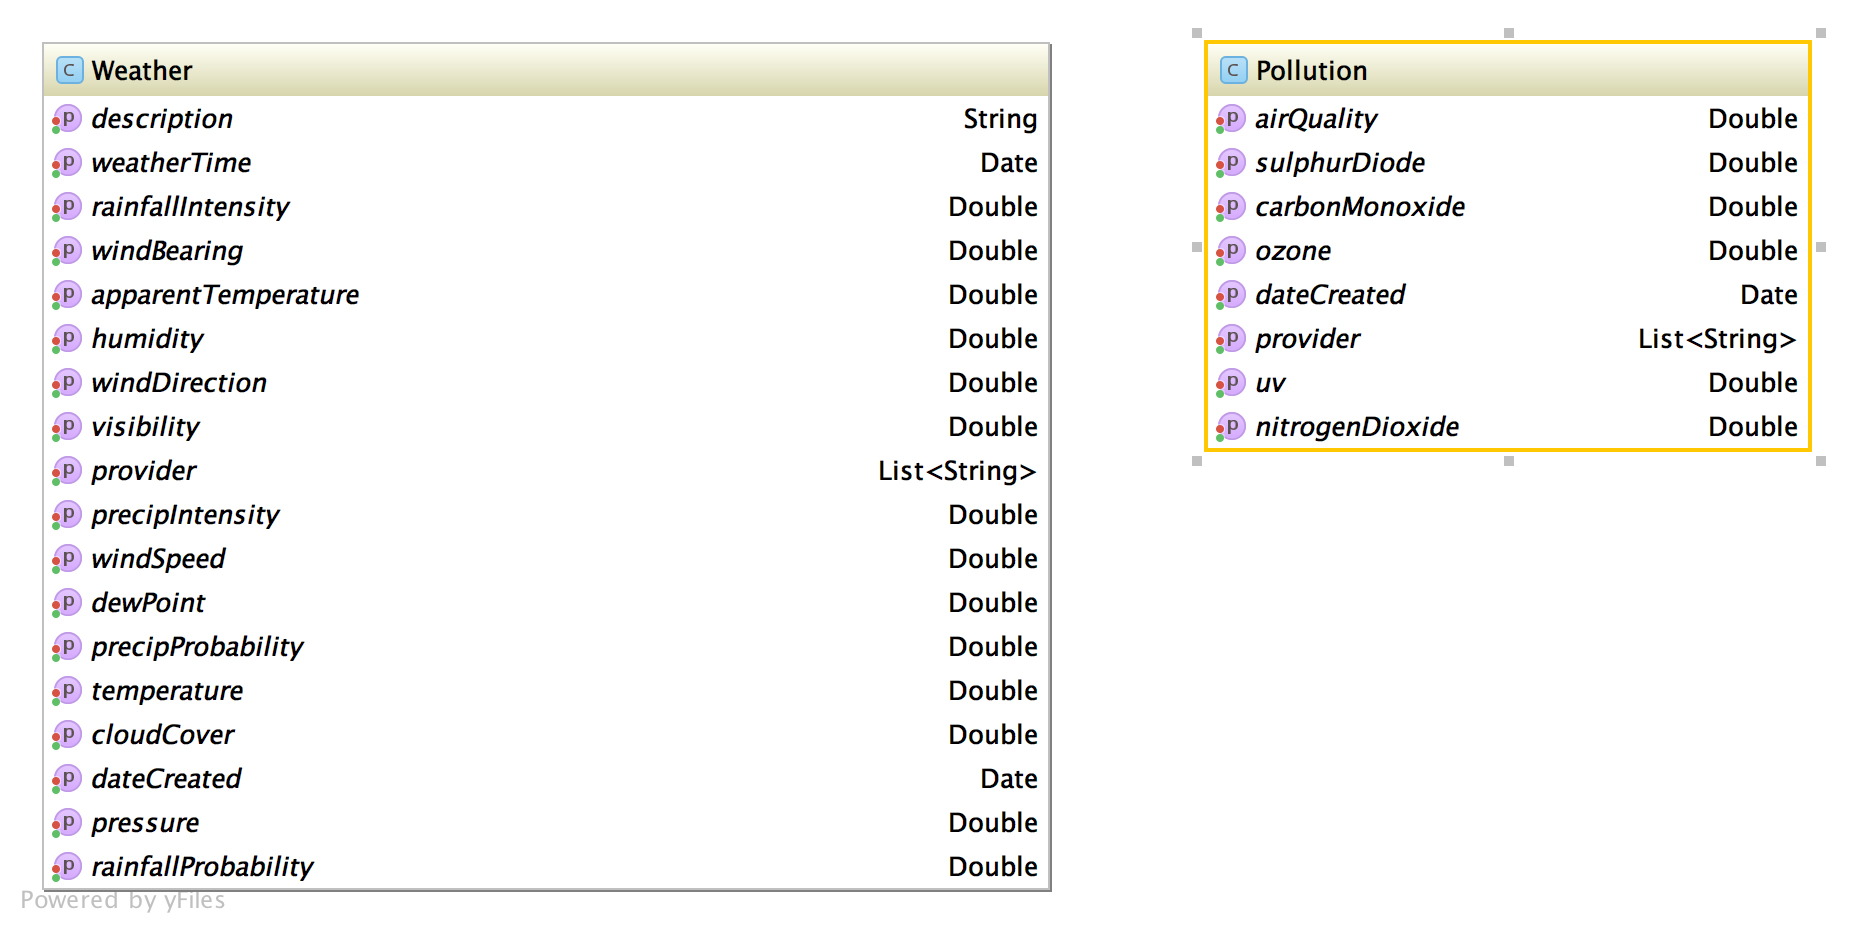
\includegraphics[width=14cm,height=10cm]{./images/SmartOwl_ClassDiagram}
      \caption{Diagrama de clases}
    \end{center}
    \end{figure}
  \newpage
  \subsection{Fuentes para la contrucción de la API}
    \paragraph{Hasta ahora se cuenta con 3 recursos principales para obtener los datos del modelo: los archivos que provee la CONAGUA (Comisión Nacional del Agua), la información de Weather Underground y la API de Forecast.io.}
     
  \subsection{Proceso de desarrollo} 
    \paragraph{Una vez que se definieron las fuentes principales para la obtención de datos se escribió una prueba que verifica la obtención de la información de cada una de ellas.} 
    \paragraph{La primera fuente de la que se extrajo información fueron los archivos que publica cada 10 minutos la página de la CONAGUA en el sitio \textbf{http://smn.cna.gob.mx/emas/}.}
    \paragraph{La técnica de Web Scraping fue utilizada para la extracción de los archivos que generan las diferentes estaciones ubicadas en los estados de las república.}
    \paragraph{Para ello se busco la url de cada archivo generado en todas las estaciones del país con ayuda de la biblioteca \textbf{tagsoup}.}
    \paragraph{Después de obtener las urls se persistieron en una base de datos no relacional de tipo llave-valor, en donde la llave es el valor de la latitud y longitud de la estación que genera la información}
    \begin{figure}[b!]
    \begin{center}
      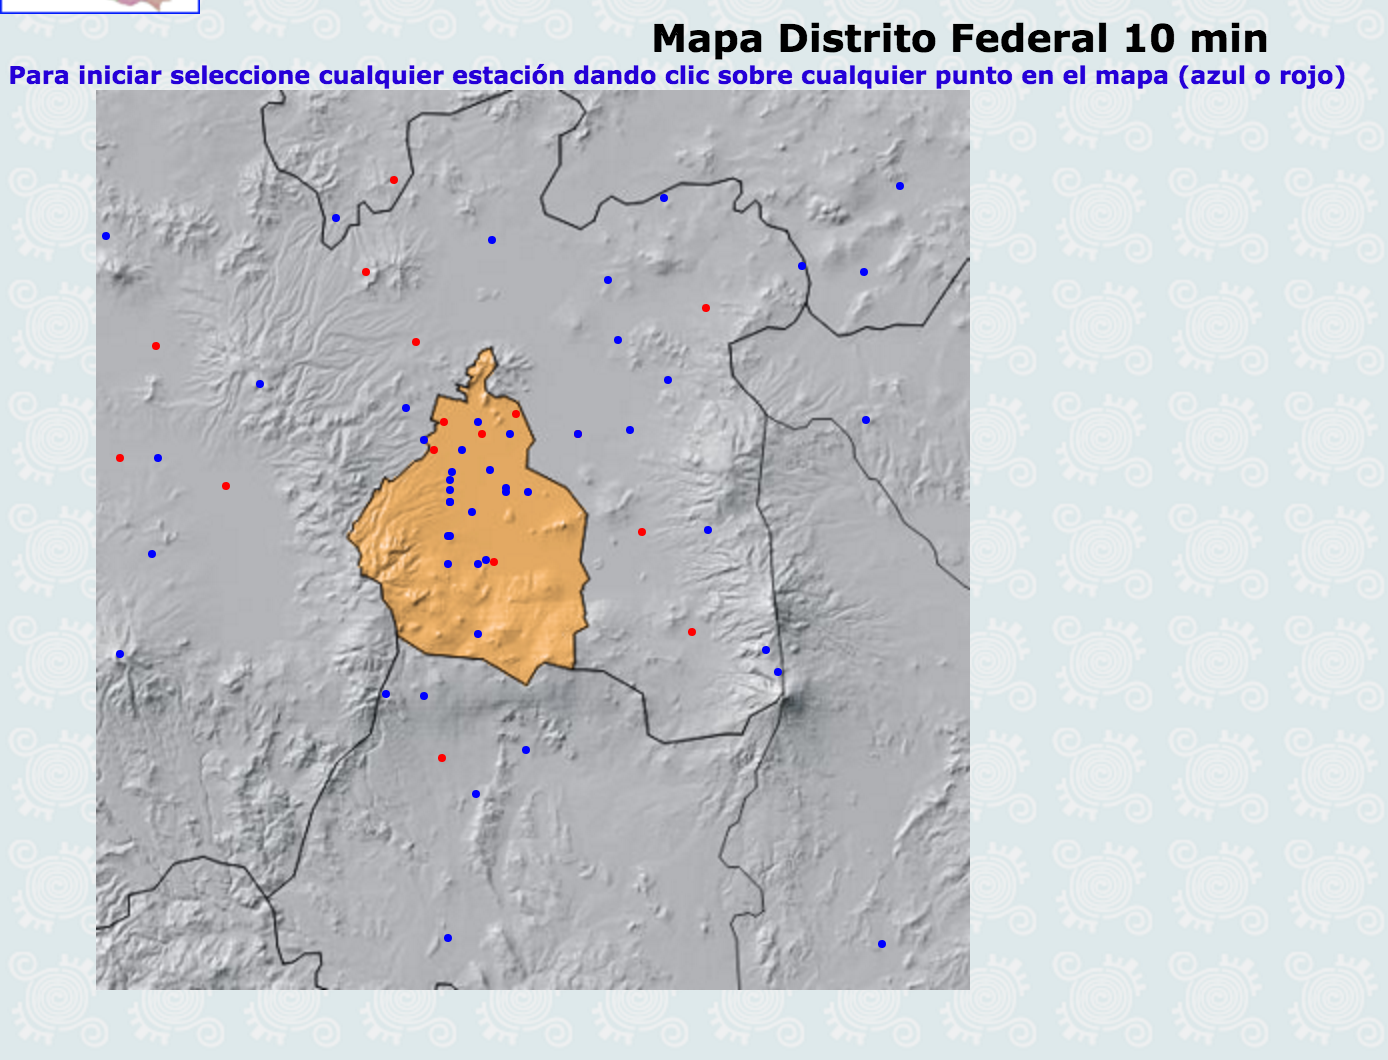
\includegraphics[width=14cm,height=10cm]{./images/DF_Stations}
      \caption{Estaciones con información climática del Distrito Federal}
    \end{center}
    \end{figure}
    \paragraph{Este proceso se ejecuta una sola vez en la aplicación, ya que cuando se despliega se verifica que ya existan las urls de los archivos en la base de datos}
    \paragraph{Ya que se tienen la información de los archivos disponible, se toma busca en la base la url del que tenga la latitud y longitud más cercana a los parámetros de consulta de la API para descargarlo y posteriormente iniciar el proceso extracción de las variables} 
    \paragraph{La segunda fuente con la que se intenta complementar el modelo es Weather Underground.}
    \paragraph{Este sitio expone un servicio que recibe un código de ciudad para obtener la información climática.}
    \begin{figure}[b!]
    \begin{center}
      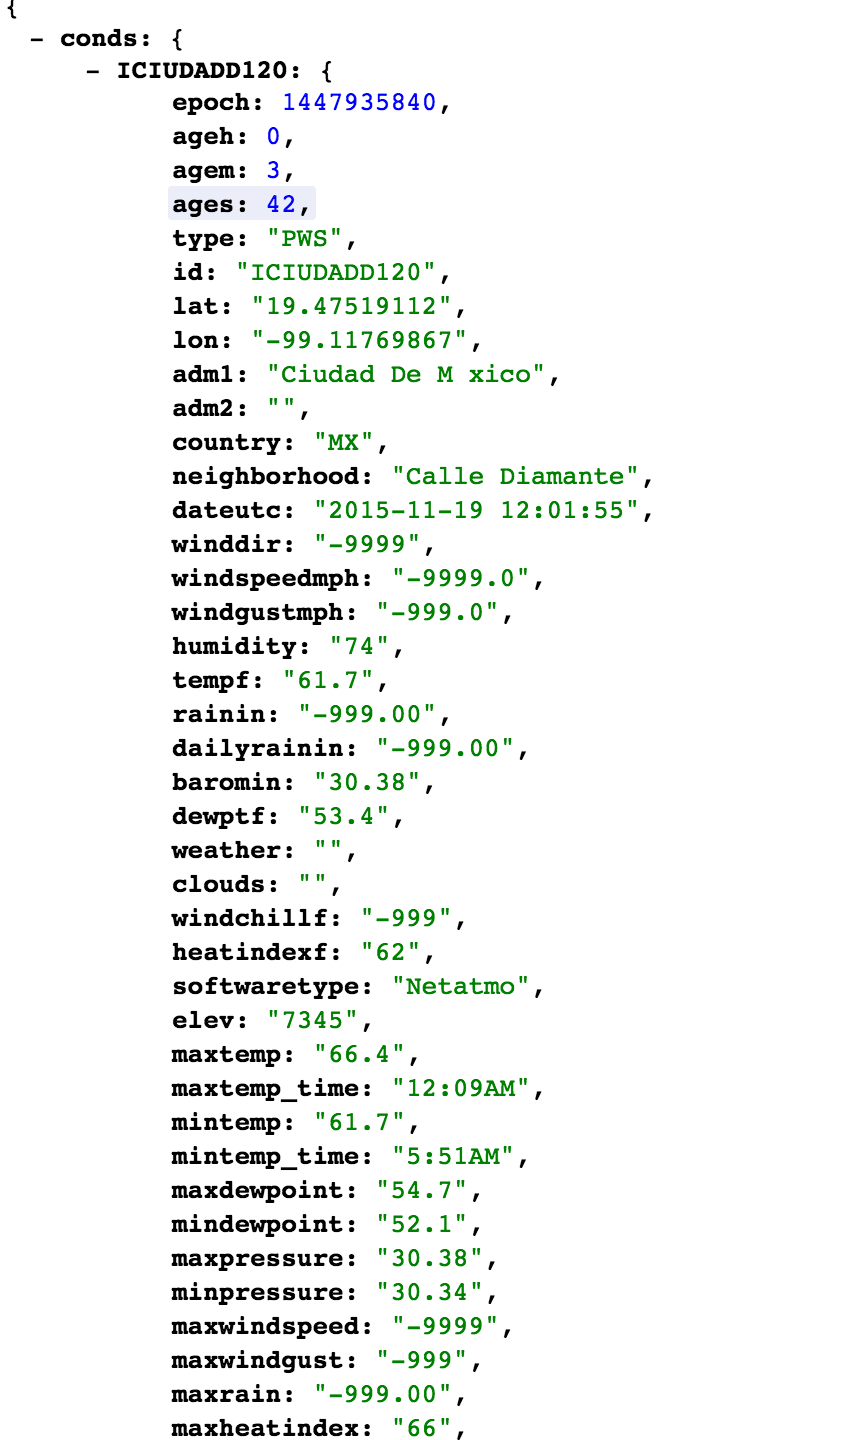
\includegraphics[width=12cm,height=17cm]{./images/WeatherUnderground}
      \caption{Consulta al servicio de WeatherUnderground}
    \end{center}
    \end{figure}
    \paragraph{Finalmente, si el modelo de datos aún no está completo, se consulta a la API de Forecast.io para buscar los datos faltantes. Esta es la última opción de búsqueda ya que la API tiene un número limitado de consultas por día.}


  \subsection{Dificultades}
    \paragraph{El desarrollo del módulo tuvo su complejidad en la obtención de los datos en las diferentes fuentes 
las fuentes de datos que tienen estructuras muy variadas, por lo que para tener un primer avance se han programado las pruebas unitarias y la funcionalidad para la extracción y estandarización de la información de cada fuente.}
  

  \subsection{Tecnologías de desarrollo}
  \paragraph{Para el desarrollo del módulo se hizo uso del lenguaje de programación Groovy.} 

  \paragraph{Smart Owl es un microservicio que se despliega con ayuda de SpringBoot y expone dos urls: /weather y /pollution que reciben los parámetros \textbf{latitude} y \textbf{longitude} para la búsqueda de la información.}

  \paragraph{Se escribió un conjunto de pruebas unitarias para la funcionalidad de la obtención de datos y la estandarización de la información con la ayuda de Spock Framework.}
  \paragraph{Gradle fue útli para las tareas de testing, administración de dependencias y la implementación del framework SpringBoot para el despliegue de la aplicación.}

  \newpage
  \begin{landscape}
      \subsubsection{Diagrama por bloques.}
        \paragraph{A continuación se mostrará el diagrama por bloques que define la estructura de Smart Owl.}
        \begin{figure}[b!]
        \centering
        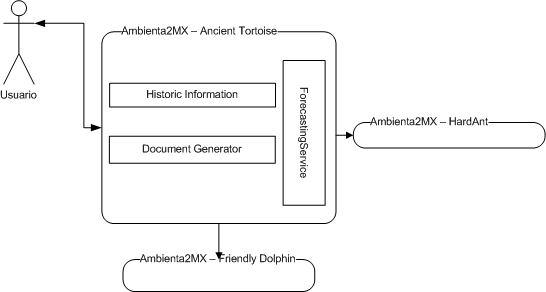
\includegraphics[width=22.5cm,height=12cm]{./images/DiagramaAncientTortoise.png}
        \caption{Diagrama General de Smart Owl}
      \end{figure}
      \end{landscape}
      \newpage
    \paragraph{A continuación se muestran los diagramas de secuencia planteados para el funcionamiento del módulo mencionado.}
    \begin{center}
      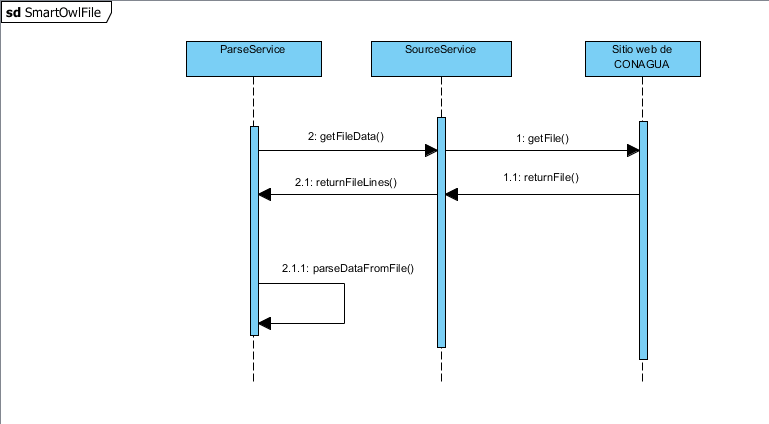
\includegraphics[width=14cm,height=9cm]{./images/SmartOwlSequenceDiagram}
    \end{center}
    \begin{center}
      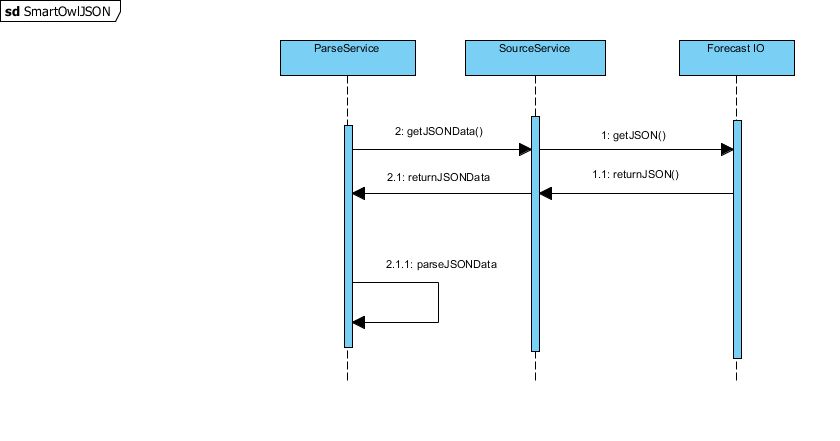
\includegraphics[width=14cm,height=9cm]{./images/SmartOwlSequenceDiagram2}
    \end{center}
    \subsubsection{Diagrama por bloques}

    \subsection{Fast Eagle}
    \subsubsection{Definición}
      \paragraph{El módulo Fast Eagle formará parte de la arquitectura final de Ambienta2MX. El propósito principal de este módulo es brindar la información cartográfica de México por medio de un servicio expuesto, considerando latitud, longitud o nombre de la localidad deseada.}
      \paragraph{Fast Eagle se encargará de exposición de datos brindados por el (Instituto Nacional de Estadística y Geografía) INEGI considerando los datos públicos que tiene de la cartografía del territorio nacional.}
      \paragraph{Actualmente la información que proporciona el INEGI se encuentra en archivos de tipo CSV o bien, terceros se han encargado de estandarizar la información de forma relacional considerando MySQL como gestor principal de información.}
      \paragraph{Sin embargo, por la necesidad de búsquedas geográficas, se generó una migración de la información a un modelo de datos orientado a documentos, siguiendo la especificación GeoJSON en su versión del año 2008. Sólo basta con realizar un proceso de exportación al gestor de de documentos Mongo, y generar los índices geográficos. \cite{35}}
      \paragraph{La información que proporciona el INEGI carece de campos esenciales para la estandarización de la información cartográfica considerando el formato propuesto por el equipo de trabajo, para dar solución a ese contratiempo se hará uso de servicios externos que ya cuentan con información definida, es decir, que su información ha pasado bajo un cierto proceso de limpieza y regulación, por ejemplo, los servicios de Google Places API.}
      \paragraph{El objetivo principal de este módulo es brindar a los demás componentes del sistema información cartográfica de una localidad de país, considerando como valores de entrada, latitud y longitud o bien el nombre del lugar.}
      \paragraph{En caso de que no exista la información deseada por el usuario o algún otro módulo del sistema en la cartografía (base de datos llamada Places), Fast Eagle tratará de resolver la información en fuentes externas, persistiendo el modelo resuelto y regresando esa información al solicitante.}
    \subsubsection{Diagrama de clases}
    \begin{center}
      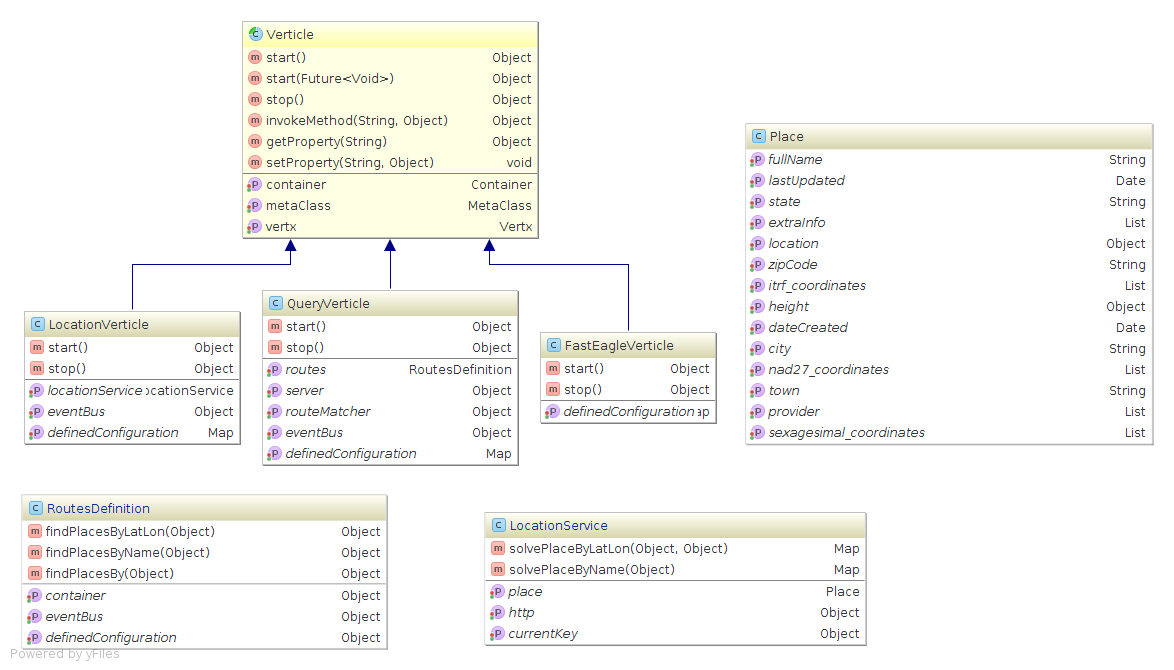
\includegraphics[width=16cm,height=10cm]{./images/FastEagleClassDiagram.png}
    \end{center}
    \newpage
    \subsubsection{Diagrama de sequencias}
    \begin{center}
      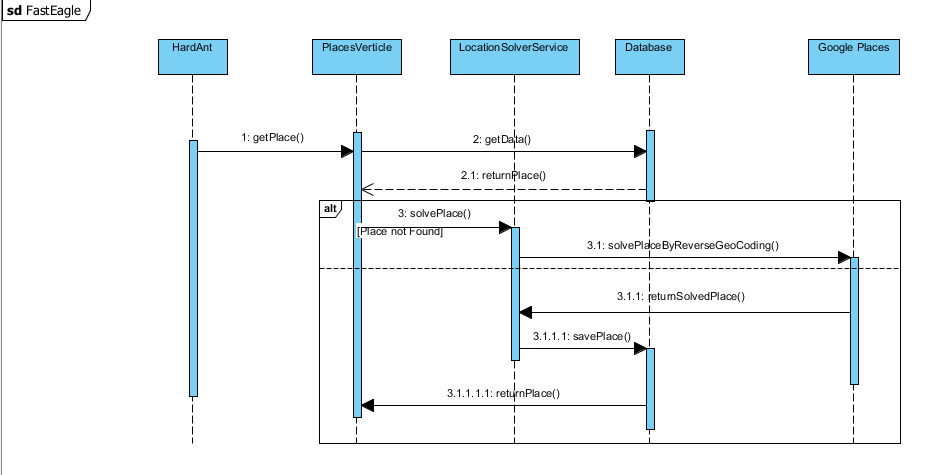
\includegraphics[width=16cm,height=10cm]{./images/FastEagleSequenceDiagram}
    \end{center}
    \subsubsection{Diagrama de bloques}
      \paragraph{Fast Eagle contará con varios procesos a ser desarrollados, la integración de cada proceso y su respectiva integración dará solución a un problema de estandarización, resolución y consulta de datos geográficos vía Latitud, Longitud y Ubicación.}
    \newpage
      \begin{landscape}
        \begin{figure}[b!]
        \centering
        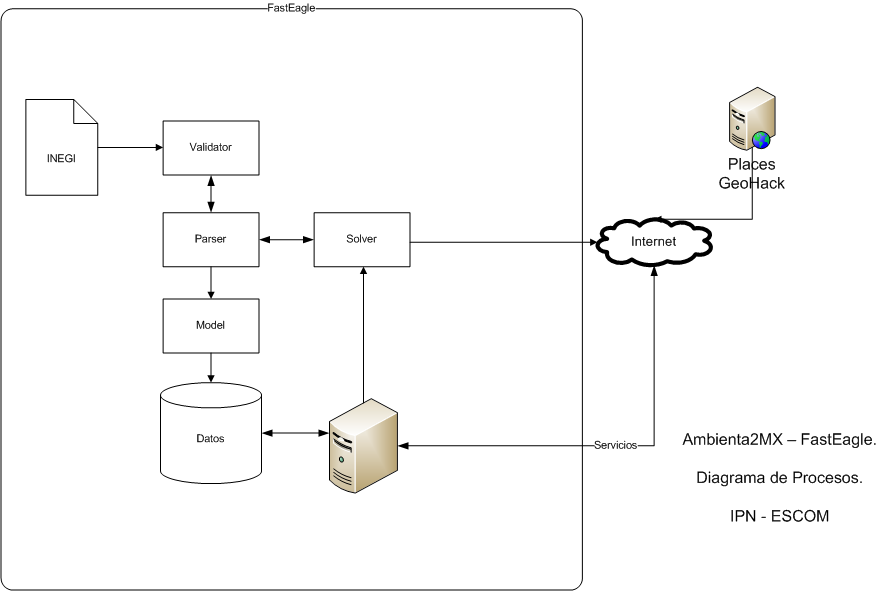
\includegraphics[width=22.5cm,height=12cm]{./images/DiagramaFastEagle.png}
        \caption{Diagrama por bloques de Fast Eagle}
      \end{figure}
      \end{landscape}
    \newpage
    \paragraph{En el diagrama se muestran tres módulos básicos, estos forman parte del núcleo de Fast Eagle, también podemos observar que se cuenta con la interacción de servicios de terceros como Google Places,  también se cuenta con la exposición de los servicios a través de un servidor web.}
    \paragraph{\textbf{\emph{Parser}} tomará los datos que el proceso de validación le arroje para transformar al estado propuesto por el equipo de trabajo (Véase modelo de datos). Considerando un proceso de resolución en caso de que la información proporcionada por el INEGI se encuentre incompleta no sea válida.}
    \paragraph{Para toda la información que carezca de datos correctos \textbf{\emph{Solver}} buscará una resolución en servicios de terceros, después de la resolución, los datos serán guardados en el gestor de bases de datos bajo el formato propuesto por el equipo de trabajo.}
    \paragraph{\textbf{\emph{Model}} es la capa de interacción con la base de datos, ésta se encarga de las operaciones mejor conocidas como CRUD (Create, Read, Update and Delete),  persistiendo la información en MongoDB, utilizando los canales de Vert.x para su convivencia con la antes mencionada.}
    \paragraph{Para poder exponer los datos, se hará uso de un servidor web minimalista orientado a micro servicios desarrollado en Vert.x, éste será un servicio público que formará parte de la infraestructura final de Ambienta2MX.}
    \paragraph{El servicio expuesto se encargará de las búsquedas a nivel base de datos y en caso de no encontrar la información buscará en terceros para poder agregarla a la base de datos y así ir mejorando el contenido de nuestro índice cartográfico.}
    \paragraph{Considerando las bondades que nos brinda el framework Vert.x, se generó un canal para la resolución de la información utilizando el servicio de Google Maps, éste canal interactua de forma directa con el servicio de places expuesto a todos los usuarios o módulos del sistema.}
    \paragraph{La comunicació principal será de tipo REST, para el proceso de obtención de información relacionada al territorio nacional.}
    \section{Hard Ant}
  \subsection{Definición y objetivos}    
    \paragraph{Hard Ant es uno de los bloques funcionales base de Ambienta2MX, su función principal es la de enrutar las peticiones a las bases de tipo MX además de brindar la solución cartográfica (a nivel ubicación) interactuando con Fast Eagle (véase Figura 8.16).}
    \begin{figure}[h!]
        \centering
          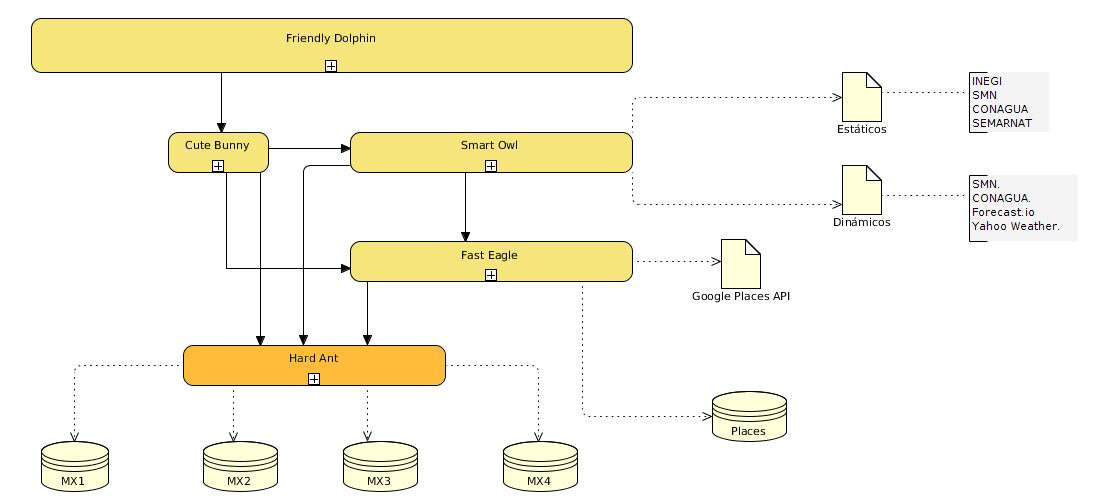
\includegraphics[width=\textwidth]{./images/DiagramaAmbienta2MX_HardAnt.png}
        \caption{Hard Ant, Módulo de Ambienta2MX.}
    \end{figure}
    \paragraph{Como complemento a la arquitectura, también contará con el proceso del registro masivo de información, exponiendo servicios que el módulo Smart Owl usará de forma constante para persistir la información estandarizada de diversas fuentes de información.}
    \paragraph{Hard Ant tiene como objetivo brindar los canales de acceso a las bases MX definidas en el diagrama general mediante servicios HTTP, estos servicios cumplen con la tarea de inserción y extracción de la información. }
    \paragraph{Este módulo es lo que sería considerado la capa del modelo de datos en un patrón MVC, ya que es la que tiene contacto de forma directa con los datos almacenados en las bases de datos orientadas a documentos gestionadas por Mongo.}
  \subsection{Alcances}
    \paragraph{Hard Ant fue diseñado para poder satisfacer la demanda en las cuatro bases de datos distrubidas, contando con un índice que se encarga de enviar la consulta a una base definda con base en la ubicación que le proporciona Fast Eagle.}
    \paragraph{Éste módulo también cuenta con la tarea de la generación de archivos de tipo CSV y JSON, que pueden ser utilizados para los fines que el usuario requiera. Todos los accesos realizarán mediante servicios de tipo REST siguiendo una Convención sobre configuración.} 
    \paragraph{Se utilizará un pool de conexiones a la base para garantizar el acceso o escritura a los datos además de brindar la posibilidad de respuestas asincronas y no bloqueantes entre las consultas realizadas.}
  \subsection{Restricciones}
    \paragraph{Para nuestro caso de estudio sólo se toma la información de la base de MX4, debido a que es la que contiene la información del Distrito Federal. Una de las limitantes más grandes es el consumo de memoria para la generación de archivos ya qué en principio se guardan de forma temporal y luego son enviados al cliente. La infraestructura que estamos manejando es limitada en recursos debido a que es gratuita.}
  \subsection{Arquitectura}
    \paragraph{A continuación se mostrará el de clases que define la estructura de Hard Ant.}
      \begin{figure}[b!]
        \centering
        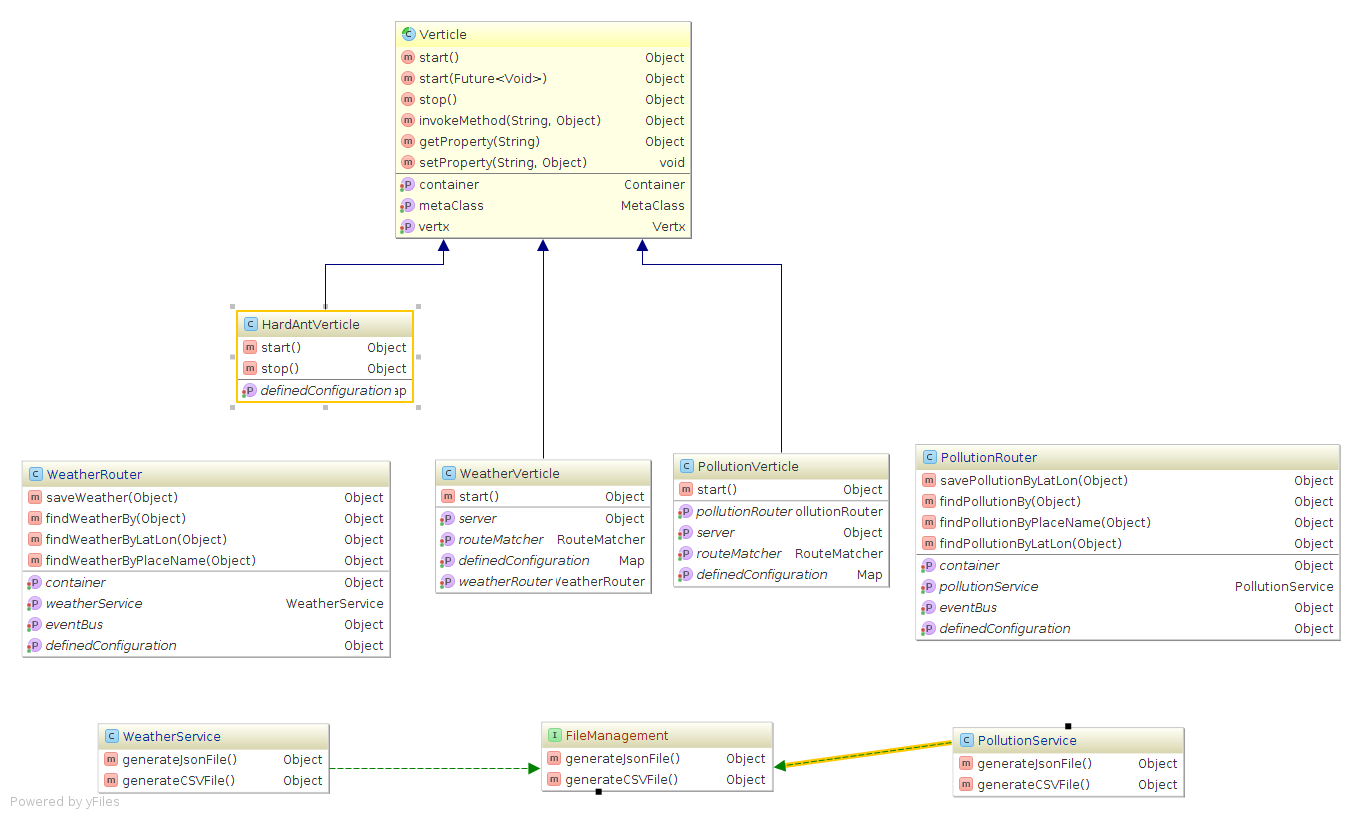
\includegraphics[width=\textwidth]{./images/HardAntClassDiagram.png}
        \caption{Diagrama de clases de Hard Ant}
      \end{figure}
    \paragraph{Las clases mostradas se ven reflejadas en el uso y adaptación de ``Verticles'', que son los componentes que se encargarán de atender peticiones, ya sea vía servicios REST o por comunicación mediante canales (Sockets), cómo se muestra en el siguiente diagrama a bloques.}
      \begin{figure}[b!]
        \centering
        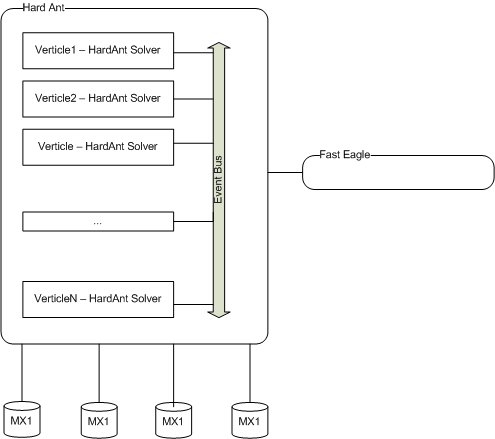
\includegraphics[width=\textwidth]{./images/DiagramaHardAnt.png}
        \caption{Diagrama a bloques de Hard Ant}
      \end{figure}
    \paragraph{En el diagrama se puede apreciar la replicación de ``Verticles'' que interactúan a través del mismo canal de información, esto brinda disponibilidad del servicio ya que las peticiones son atendidas y procesadas no sólo por un elemento existente si no varios (véase Figura 8.17). La interacción con este servicio se realizará utilizando servicios REST, utilizando el módulo de Cute Bunny como medio de comunicación con la vista que tendrá el usuario final.}
    \paragraph{Considerando trabajos más pesados (Obtención de datos climáticos considerando un radio, cadena de búsqueda o bien información de un punto definido) se utilizarán procesos en segundo plano, esto es posible gracias a la implementación de ``Verticles'' nativas de Vert.x, tecnología que será usada para el desarrollo y despliegue final de éste módulo.}
    \paragraph{Actualmente se propone el despliegue de varias ``Verticles'', además de las que el mismo framework despliega para el consumo de las bases de datos \cite{33}.Quedando en ocho, cuatro encargadas de la comunicación y distribución de la información y las cuatro restantes para atender peticiones (véase Figura 8.18).} 
    \paragraph{De forma específica, también se hará uso de los canales implementados por Vert.x para generar una comunicación con las bases de datos con la finalidad de poder generar la distribución de estas. Los canales podrían ser accedidos siempre y cuando se pertenezca a la misma red o bien al cluster de Vert.x, esta modalidad no ha sido habilitada por cuestiones de seguridad.}
  \subsection{Factibilidad} 
    \paragraph{Considerando el mismo modo de trabajo que en }
  \subsection{Implementación}
    \paragraph{Hablando más a detalle, Hard Ant, puede ser desplegado utilizando la línea de comandos gracias a las funciones que nos provee Gradle, framework utilizado para el maquetado, resolución de dependencias y gestión de tareas del proyecto. \cite{34}}
    \paragraph{El código y el proyecto como tal se encuentran en línea utilizando Git\cite{38} en conjunto con Github\cite{39}, para el proceso de control de versiones (véase Figura 8.19). Para la gestión de tareas y desarrollo del proyecto fue utilizado Gradle en conjunton con Vert.x.}
    \paragraph{Las ventajas que nos ofrece Git/Github es la integración con procesos de desarrollo utilizando metodologías ágiles. La siguiente imagen muestra el control y manejo de issues (análogos a objetivos o features) que fueron desarrollados para cumplir con los objetivos y mejoras planteadas para cada módulo.}
    \begin{figure}[h!]
        \centering
          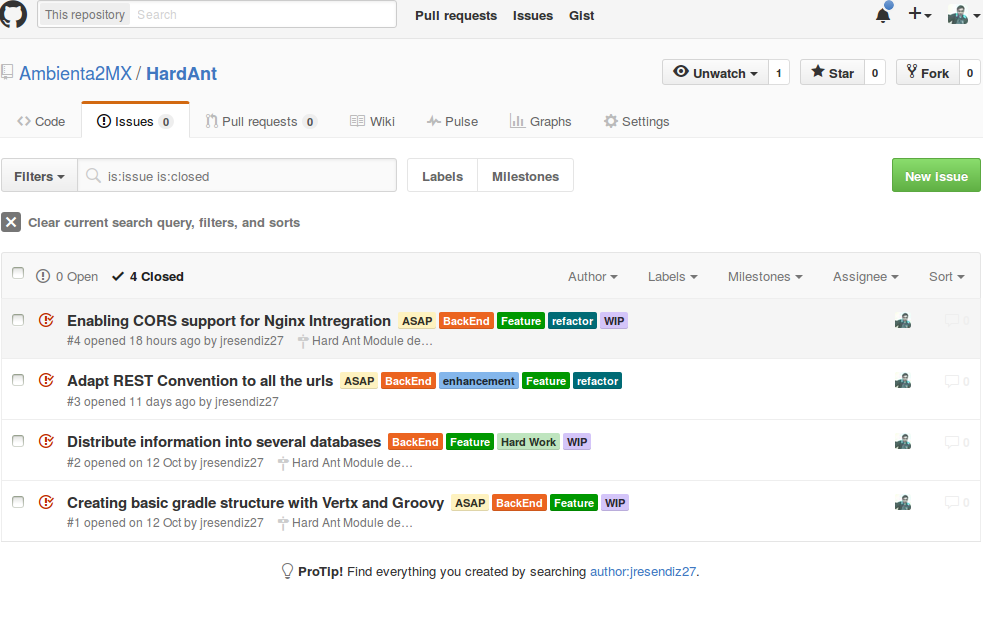
\includegraphics[width=\textwidth]{./images/HardAntIssues.png}
          \caption{Hard Ant, Integración con Github.}
    \end{figure}
    \paragraph{Este módulo se puede encontrar en cualquier otra máquina, debido al método de comunicación utilizado entre los módulos, sólo basta con realizar la configuración de las direcciones o dominios donde se encuentra alojado para qué este puede pueda ser accedido.}
  \subsection{Pruebas y Capturas de pantalla}
    \paragraph{A continuación se muestran algunas pruebas realizadas y las capturas de pantalla del servicio REST y la respuesta qué este nos regresa.}
      \begin{figure}[h!]
        \centering
          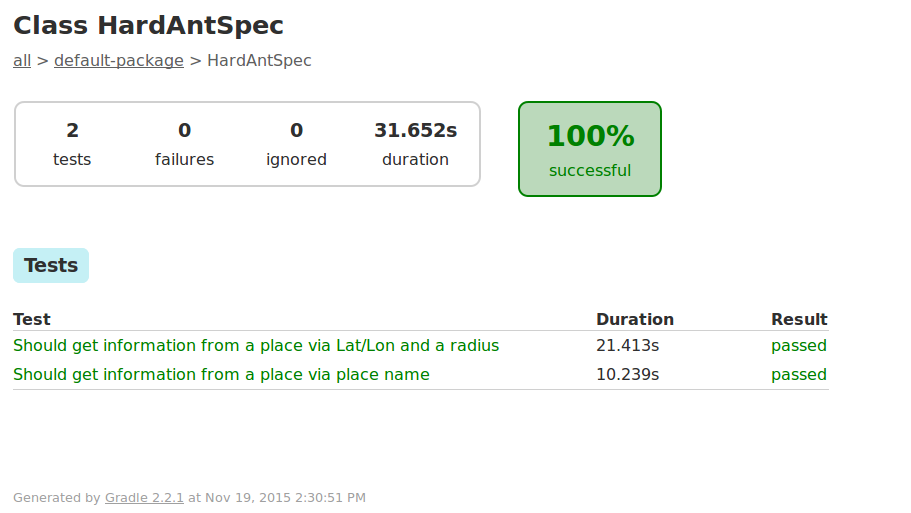
\includegraphics[width=\textwidth]{./images/PruebasHardAnt}
          \caption{Hard Ant, Pruebas unitarias.}
      \end{figure}
      \begin{figure}[h!]
        \centering
          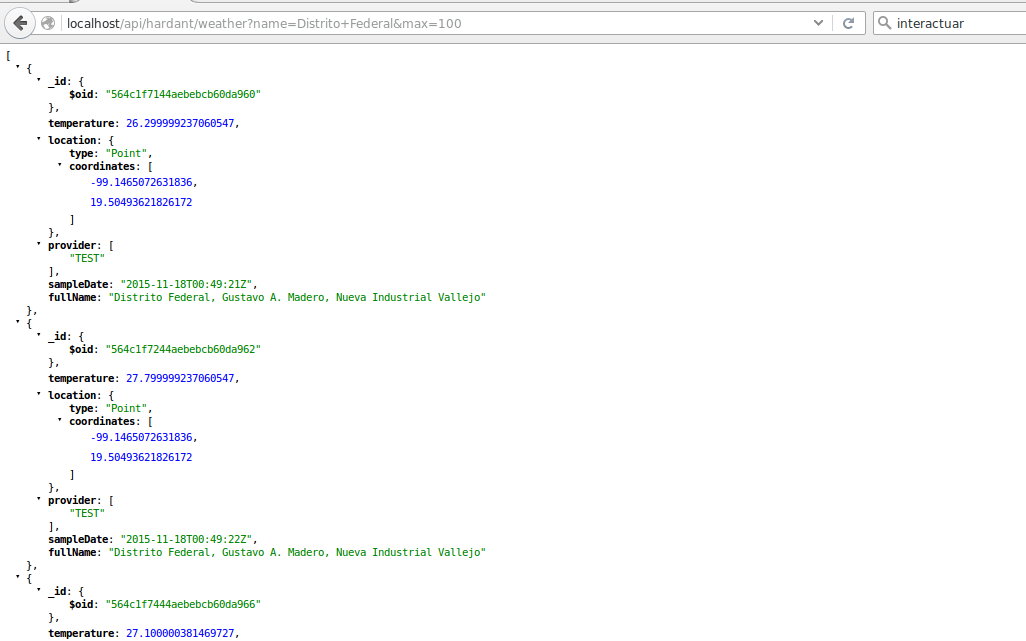
\includegraphics[width=\textwidth]{./images/CapturaHardAnt}
          \caption{Hard Ant, Respuesta del servicio rest.}
      \end{figure}

